\section{Introdução}
\bibliographystyle{plainnat}

\subsection{Desafios}
\begin{frame}\frametitle{Introdução}

  \begin{tabular}{cc}  
    \begin{tabular}{c}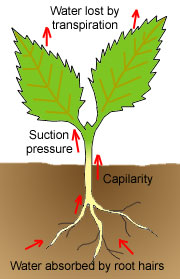
\includegraphics[height=3.5cm]{transp}\end{tabular} & 
  \begin{tabular}{c}\parbox{0.5\linewidth}{Desenvolvimento e produção \\ \centering{$\equiv$} \\ transpiração da planta}\end{tabular}  
    \\
    \begin{tabular}{c}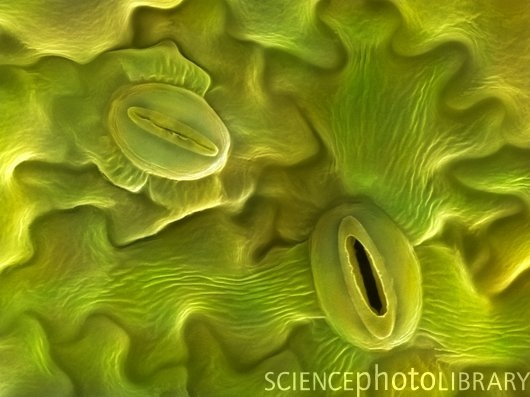
\includegraphics[height=2cm]{stomata}\end{tabular} &
  \begin{tabular}{c}\parbox{0.5\linewidth}{
      Estresse (biótico/abiótico) \\ \centering{$\downarrow$} \\ Fechamento dos estômatos \\ $\downarrow$ \\ Alteração na transpiração
  }\end{tabular} 
    \\
\end{tabular}
\end{frame}

\subsection{Desafios da modelagem}
\begin{frame}\frametitle{Introdução}
  \begin{itemize}
    \item Encontrar um modelo que explique suficientemente bem o fenomeno para o propósito escolhido;
    \item Relação número de parâmetros/grau de complexidade do modelo difícil de ser ajustado;
    \item Encontrar simplificações que tornem a resolução possível, perdendo o mínimo possível de precisão \\ (realidade X simulação). \\~\\
  \end{itemize}
  \centering{Modelagem $\rightarrow$ entender/simular/prever os fenômenos \\ $\downarrow$ \\ melhorar práticas de manejo das culturas}
\end{frame}

\subsection{Revisão}
\begin{frame}\frametitle{Extração de soluto}
  \scriptsize 
  \begin{block}{Modelos macroscópicos}
    {\scriptsize 
      Considera toda a zona radicular como um componente de extração uniforme.

      A extração de água e soluto é um termo ``sumidouro'' nas equações de balanço de massa.
    }
  \end{block}
  \begin{block}{Modelos microscópicos}
    {\scriptsize 
      Considera uma raiz singular cinlíndrica de raio e propriedades de extração uniformes.

      A extração de água e solutos são determinadas pelas condições de contorno das equações de balanço de massa à superfície da raíz.
    }
  \end{block} \pause
  \begin{block}{Solução numérica X Solução analítica}
  \end{block}
  \bgroup
  \def\arraystretch{1.5}
  \begin{tabular}{cc}
    \scriptsize Numérica & \scriptsize Analítica \\
    \tiny
\(
 \begin{bmatrix}
 b_1 & c_1 & & & &  \\
 a_2 & b_2 & c_2 & & &  \\
  & a_3 & b_3 & c_3 & &  \\
  &  & \ddots & \ddots & \ddots &  \\
  &  & & a_{n-1} & b_{n-1} & c_{n-1}  \\
  &  & & & a_{n} & b_{n}  \cr \end{bmatrix}
 \begin{bmatrix}
 C^{j+1}_1 \\
 C^{j+1}_2 \\
 C^{j+1}_3 \\
 \vdots \\
 C^{j+1}_{n-1} \\
 C^{j+1}_n \\ \end{bmatrix}
=
 \begin{bmatrix}
 f_1 \\
 f_2 \\
 f_3 \\
 \vdots \\
 f_{n-1} \\
 f_n \\ \end{bmatrix}
\)
 & 
\tiny\(
\Theta(\mu,\eta) = \sum_{n=0}^\infty A_n \mu^v \beta_v(\mu,\tau,\alpha_n) \exp(-\alpha_n^2\eta)+1
\)    \\
  \end{tabular}
  \egroup
\end{frame}

%\subsection{Revisão}
\begin{frame}\frametitle{Soluções existentes}
    \begin{itemize}
    \item Início $\rightarrow$ soluções analíticas em regime estacionário para o fluxo de água e solutos
    \item Computadores $\rightarrow$ soluções numéricas uni, bi e tridimensionais (regime transiente)
      \begin{itemize}
	\item soluções com extração de soluto linear ou não-linear
      \end{itemize}
  \end{itemize}
  \centering
  Possibilidade de prever o estresse hídrico e osmótico
  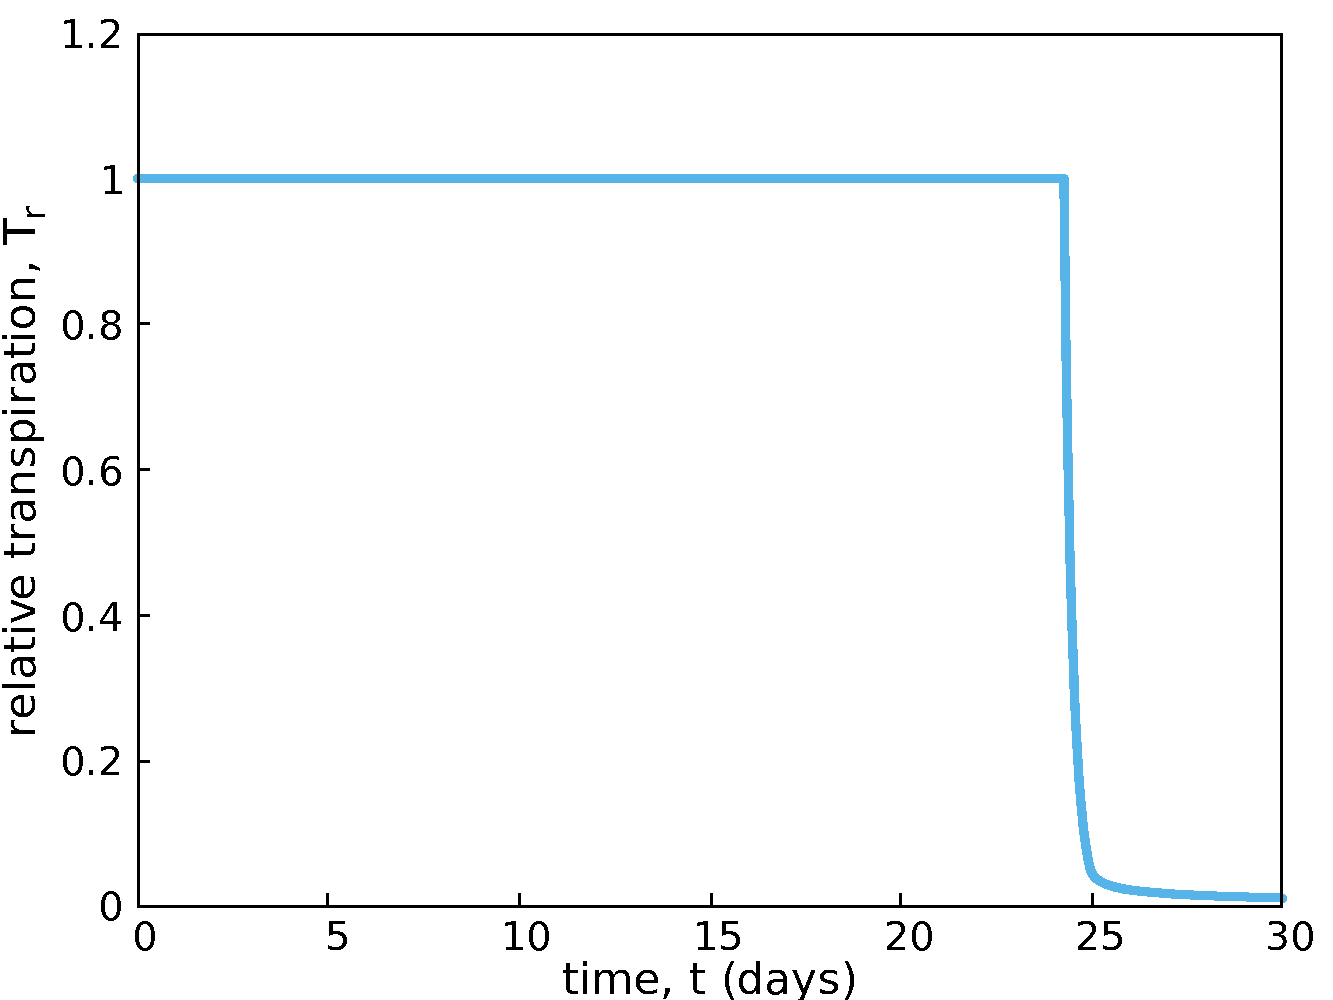
\includegraphics[height=2.5cm]{tr_pres}\\
\end{frame}

\subsection{Soluções existentes}
\scriptsize
\begin{frame}
  \begin{block}{Modelos empíricos}
    \cite{feddes78}, \cite{homaee}, Li et al. (2006)

    Redução da transpiração $\rightarrow$ parâmetros empíricos

    \centering
    \begin{tabular}{cc}
      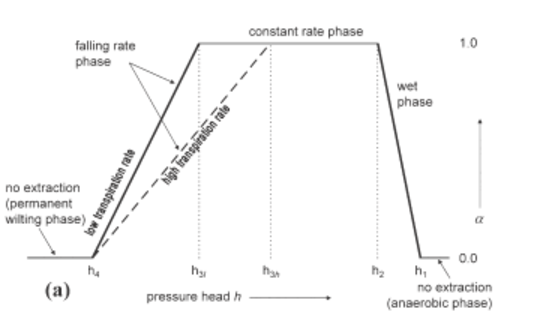
\includegraphics[height=2.5cm]{Ftr} &
      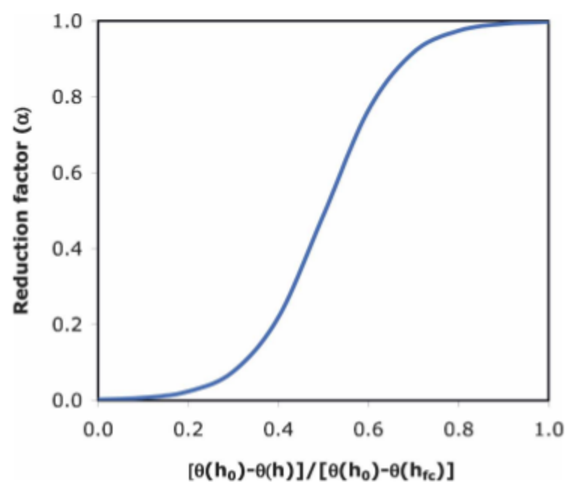
\includegraphics[height=2.5cm]{Ltr} \\
    \end{tabular}
  \end{block}
  
  \begin{block}{Modelo mecanístico}
    \cite{liersolute}

    Redução da transpiração $\rightarrow$ potencial hídrico limitante (LER TRABALHO DE QUIRIJN Q FALA COMO SE OBTER $h_lim$)
    
    \centering
    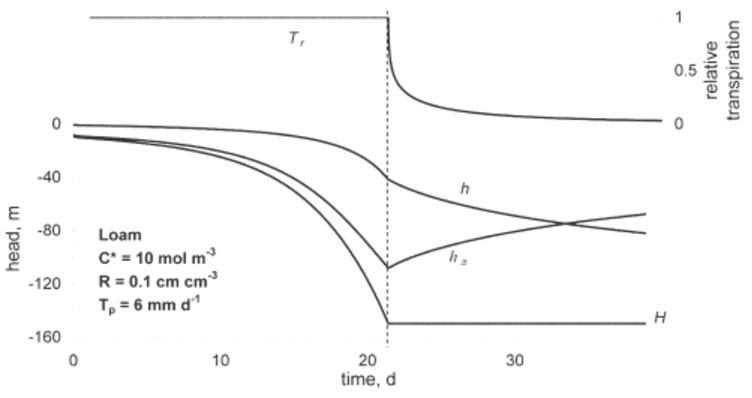
\includegraphics[height=2.5cm]{Qtr}
  \end{block}
\end{frame}


\subsection{Solução proposta - REDUZIR TEXTO}
  
\begin{frame}\frametitle{Solução proposta}
  Modelo microscópico, numérico e mecanístico com extração não-linear de soluto (dependente da concentração do solo) \\[0.2cm]
  \begin{itemize}
    \item Utilizou-se como base o modelo mechanístico de extração de água e fluxo de soluto proposto por \cite{liersolute},
    \item Resolver a Equação de Convecção-Dispersão para o movimento de soluto no solo, considerando fluxos transientes de água e soluto e assumindo uma extração (não-linear) de soluto sendo depende de sua concentração no solo.
          que resolve numericamente as equações de balanço de massa, porém não considera a extração de soluto e somente o seu movimento em direção à raiz.
    \item\begin{tabular}{p{4.5cm} c}
            Buscando-se uma solução também mecanística para a extração de solutos, utilizou-se a equação de Michaelis-Menten como condição de fronteira à superfície da raiz. &
	    \raisebox{-.7\height}{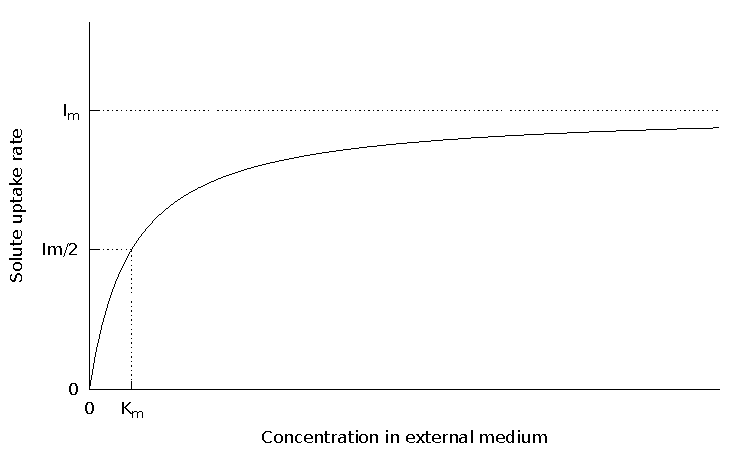
\includegraphics[height=2.5cm]{orig_MM}} \\
         \end{tabular}
  \end{itemize}
\end{frame}

%\subsection{Importância da modelagem}
%\begin{frame}\frametitle{Introdução}
%  \centering{Modelagem $\rightarrow$ entender/simular/prever os fenômenos \\ $\downarrow$ \\ melhorar práticas de manejo das culturas}
%\end{frame}

\subsection{Objetivos}
\begin{frame}\frametitle{Objetivos da Tese}
  \begin{itemize}
  \item Incorporar extração de soluto no modelo de \cite{liersolute};
  \item Diferenciar quantitativamente as componentes passiva e ativa da extração de solutos;
  \end{itemize}
  \begin{block}{Importância}
    Incorporar o modelo em uma modelo mais completo (SWAP)
  \end{block}
  MELHORAR O TEXTO (INFORMACOES)
\end{frame}


